\documentclass{article}\usepackage[]{graphicx}\usepackage[]{xcolor}
% maxwidth is the original width if it is less than linewidth
% otherwise use linewidth (to make sure the graphics do not exceed the margin)
\makeatletter
\def\maxwidth{ %
  \ifdim\Gin@nat@width>\linewidth
    \linewidth
  \else
    \Gin@nat@width
  \fi
}
\makeatother

\definecolor{fgcolor}{rgb}{0.345, 0.345, 0.345}
\newcommand{\hlnum}[1]{\textcolor[rgb]{0.686,0.059,0.569}{#1}}%
\newcommand{\hlsng}[1]{\textcolor[rgb]{0.192,0.494,0.8}{#1}}%
\newcommand{\hlcom}[1]{\textcolor[rgb]{0.678,0.584,0.686}{\textit{#1}}}%
\newcommand{\hlopt}[1]{\textcolor[rgb]{0,0,0}{#1}}%
\newcommand{\hldef}[1]{\textcolor[rgb]{0.345,0.345,0.345}{#1}}%
\newcommand{\hlkwa}[1]{\textcolor[rgb]{0.161,0.373,0.58}{\textbf{#1}}}%
\newcommand{\hlkwb}[1]{\textcolor[rgb]{0.69,0.353,0.396}{#1}}%
\newcommand{\hlkwc}[1]{\textcolor[rgb]{0.333,0.667,0.333}{#1}}%
\newcommand{\hlkwd}[1]{\textcolor[rgb]{0.737,0.353,0.396}{\textbf{#1}}}%
\let\hlipl\hlkwb

\usepackage{framed}
\makeatletter
\newenvironment{kframe}{%
 \def\at@end@of@kframe{}%
 \ifinner\ifhmode%
  \def\at@end@of@kframe{\end{minipage}}%
  \begin{minipage}{\columnwidth}%
 \fi\fi%
 \def\FrameCommand##1{\hskip\@totalleftmargin \hskip-\fboxsep
 \colorbox{shadecolor}{##1}\hskip-\fboxsep
     % There is no \\@totalrightmargin, so:
     \hskip-\linewidth \hskip-\@totalleftmargin \hskip\columnwidth}%
 \MakeFramed {\advance\hsize-\width
   \@totalleftmargin\z@ \linewidth\hsize
   \@setminipage}}%
 {\par\unskip\endMakeFramed%
 \at@end@of@kframe}
\makeatother

\definecolor{shadecolor}{rgb}{.97, .97, .97}
\definecolor{messagecolor}{rgb}{0, 0, 0}
\definecolor{warningcolor}{rgb}{1, 0, 1}
\definecolor{errorcolor}{rgb}{1, 0, 0}
\newenvironment{knitrout}{}{} % an empty environment to be redefined in TeX

\usepackage{alltt}
\usepackage{amsmath} %This allows me to use the align functionality.
                     %If you find yourself trying to replicate
                     %something you found online, ensure you're
                     %loading the necessary packages!
\usepackage{amsfonts}%Math font
\usepackage{graphicx}%For including graphics
\usepackage{hyperref}%For Hyperlinks
\usepackage[shortlabels]{enumitem}% For enumerated lists with labels specified
                                  % We had to run tlmgr_install("enumitem") in R
\hypersetup{colorlinks = true,citecolor=black} %set citations to have black (not green) color
\usepackage{natbib}        %For the bibliography
\setlength{\bibsep}{0pt plus 0.3ex}
\bibliographystyle{apalike}%For the bibliography
\usepackage[margin=0.50in]{geometry}
\usepackage{float}
\usepackage{multicol}

%fix for figures
\usepackage{caption}
\newenvironment{Figure}
  {\par\medskip\noindent\minipage{\linewidth}}
  {\endminipage\par\medskip}
\IfFileExists{upquote.sty}{\usepackage{upquote}}{}
\begin{document}

\vspace{-1in}
\title{Lab 5 -- MATH 240 -- Computational Statistics}

\author{
  Sankalp Ojha \\
  Colgate University  \\
  Mathematics  \\
  {\tt sojha@colgate.edu}
}

\date{}

\maketitle

\begin{multicols}{2}
\begin{abstract}
This study aims to answer of who contributed most to the making of the song "Allentown". Was it The Front Bottoms, All Get Out, or Manchester Orchestra? Each band's style was anaylzed and compared with the characteristics of Allentown. The study concluded that Manchester Orchestra had the most contribution followed by All Get Out as the second largest contributor. The Front Bottoms were the band which contribiuted the least to the making of Allentown.
\end{abstract}

\section{Introduction}
Through this lab, we will be exploring who contributed more to the song "Allentown". Was it The Front Bottoms, All Get Out, or Manchester Orchestra? To answer the question at hand, we will analyze all the songs released, excluding all joint albums, live albums, and single releases contained in a full album or an Extended Play (EP), by all the bands before Allentown. Through the analysis, we will aim to determine the style of each band which will allow us to compare Allentown's style with each band. The comparison will allow us to determine which band's style matches the most with Allentown, leading to the conclusion of which band contributed in a greater quantity.

\section{Methods}

\subsection{Making A batfile.txt}
To accomplish this lab, we will first need to create a \texttt{batfile.txt} file using the \texttt{R} package \texttt{stringr} \citep{stringr} that we can execute in the command line to produce a \texttt{.json} file. Using the \texttt{R} package \texttt{jsonlite} \citep{jsonlite} we will gather all relevant information needed, such as tempo in beats per minute, musical key or musical mode, to analyze the similarities between the each band's style and Allentown's style. 

To create the \texttt{batfile.txt} file, I downloaded all the given songs which were assorted by artist with a sub folder for each album. Each album folder contains all the songs in that given album. We retrieved the artist name, album name, and each track's name from the file path to create a file name for each song's \texttt{.json} file. Each song's file path and \texttt{.json} file name were pasted into an execuatble \texttt{batfile.txt} file which will be used to create the necessary \texttt{.json} file for each song.

\subsection{Gathering All Relevant Data And Merging \texttt{.csv} Files}
We used Essentia Extractor \citep{essentia} to obtain all the \texttt{.json} files for the songs. Once we had all 181 \texttt{.json} files one for each song, it was time to sift through all the data and gather all relevant information needed for our analysis. We also were provided with Essentia models \citep{essentiamodels} which came in the form of a \texttt{.csv} file. The grand outcome of this portion of the lab is to sift through the data and create a new data frame with only the relevant information we will need for the final portion of the lab which will be to analyze the data. Cleaning up the data first requires combining similar variables into one average variable. For example, for the party measurement, we took an average of the \texttt{eff party} and \texttt{nn party} variables to get a mean average party variable. We used this combining process for all the measurements we wanted to analyze at the end. The final step of compiling all the relevant information was creating a new data frame which only contained the necessary information such as artist, album, track, and all the new variables we created. We also used LIWC \citep{LIWC} to extract information about the frequency of keywords and emotions in the songs. We used the \texttt{R} function \texttt{merge()} to merge the \texttt{streaming music extractor}\texttt{.csv}, the key information\texttt{.csv} we made, and the LIWC\texttt{.csv} file. The new merged data frame will allow us to extract various pieces of information which we will be able to use for making graphs and plots for analyzing which band contributed more to the making of Allentown.

\subsection{Making A Descion}
Once, we had our master data frame, I created a \texttt{R} function which would compare each bands characteristics with Allentown's characteristics. The function finds each band's median, interquartile range (IQR), maximum, and minimum value for a given characteristic. The function finally determines whether the given characteristic is ``Within Range", Allentown's level falls within the IQR, ``Outlying", Allentown's level falls outside of the IQR but within the max and min, ``Out Of Range", Allentown's level falls outside of the max and min values. I furthered summed up the number of occurrences of the three categories each band had. I also made a points which award each band one point for being ``Within Range" and half a point for being ``Outlying". This way I could quantify the impact of falling into one of the three categories.

\section{Results}
In the appendix, there is a figure which displays four plots. Each plot shows the number of occurrences each band had for a specific label and also displays the points table. From my observations, Manchester Orchestra had the most contribution to the making of Allentown. All Get Out had the second most contribution followed by The Front Bottoms, who had the least amount of contribution.

\section{Discussion}
As can be seen in the plots, Manchester Orchestra had the most amount of `Within Range", which is a clear indicator that they had a hefty contribution. Manchester Orchestra also had the least amount of ``Out Of Range", which supports the conclusion that they had the most contribution. With the same logic, All Get Out came second both of those categories as well, which implies they had the second most amount of contribution. The points plot is also consitent with the infrence of Manchester Ochestra having the most contribition and All Get Out being the second largest contributor.

%%%%%%%%%%%%%%%%%%%%%%%%%%%%%%%%%%%%%%%%%%%%%%%%%%%%%%%%%%%%%%%%%%%%%%%%%%%%%%%%
% Bibliography
%%%%%%%%%%%%%%%%%%%%%%%%%%%%%%%%%%%%%%%%%%%%%%%%%%%%%%%%%%%%%%%%%%%%%%%%%%%%%%%%
\vspace{2em}

\begin{tiny}
\bibliography{bib5}
\end{tiny}
\end{multicols}

%%%%%%%%%%%%%%%%%%%%%%%%%%%%%%%%%%%%%%%%%%%%%%%%%%%%%%%%%%%%%%%%%%%%%%%%%%%%%%%%
% Appendix
%%%%%%%%%%%%%%%%%%%%%%%%%%%%%%%%%%%%%%%%%%%%%%%%%%%%%%%%%%%%%%%%%%%%%%%%%%%%%%%%
\newpage
\onecolumn
\section{Appendix}

\begin{figure}[H]
\begin{center}
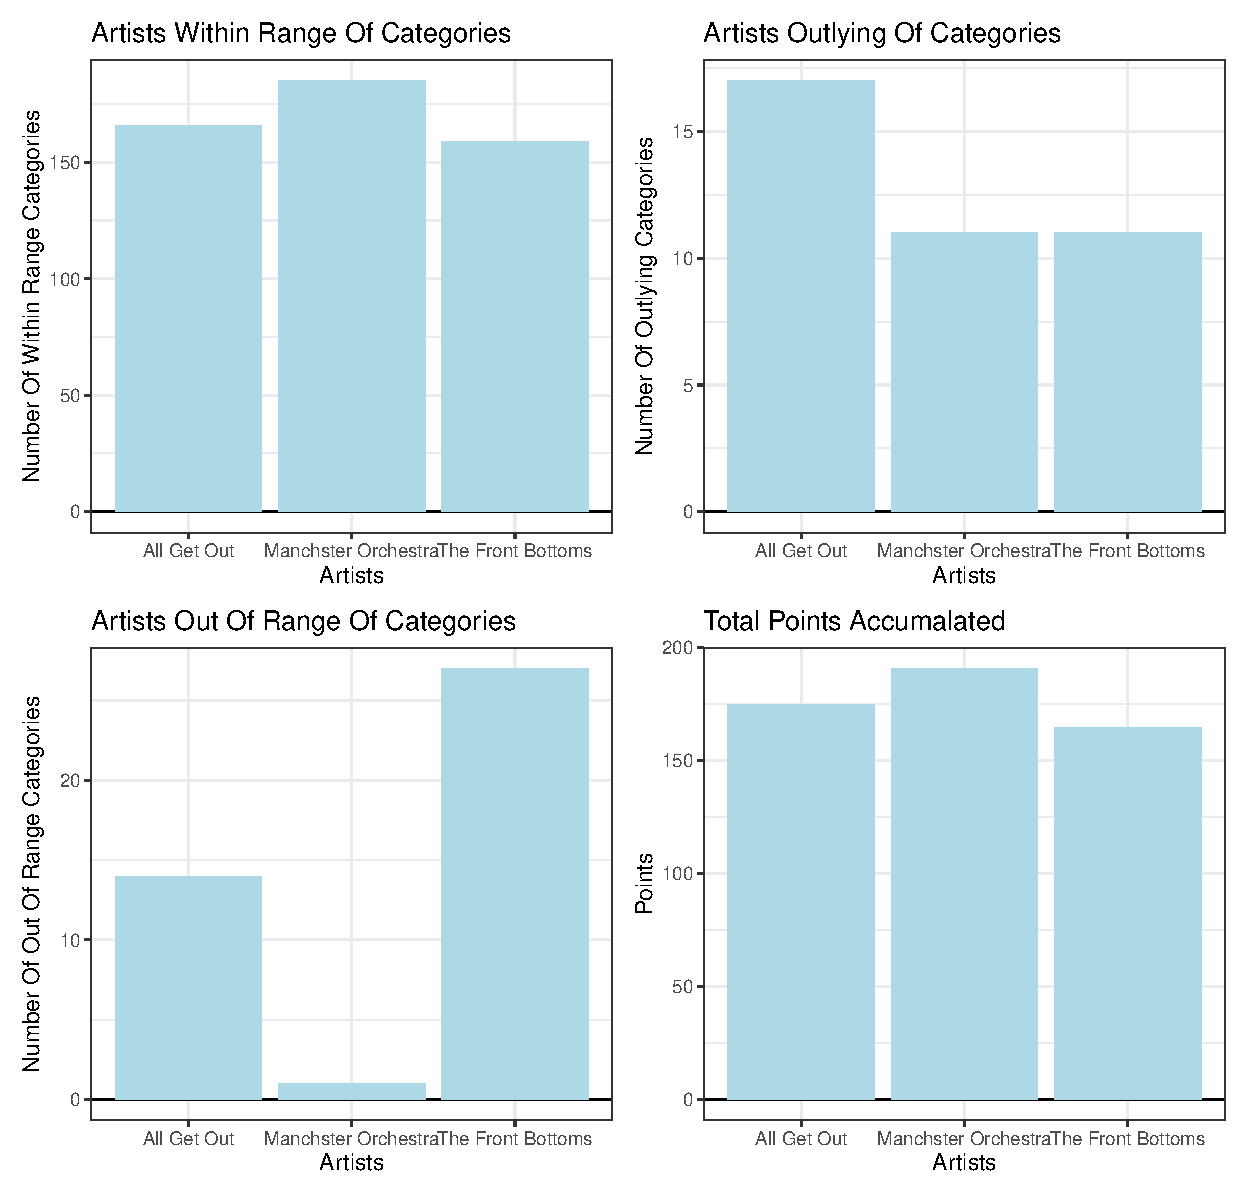
\includegraphics[scale=0.75]{Rplot.pdf}
\caption{Plots For Each Category}
\label{plot5}
\end{center}
\end{figure}

\begin{table}[ht]
\centering
\begin{tabular}{lrrrrr}
  \hline
 & artists & count.in.range & count.outlying & count.out.range & points \\ 
  \hline
1 & All Get Out & 166.00 & 17.00 & 14.00 & 174.50 \\ 
2 & Manchester Orchestra & 185.00 & 11.00 & 1.00 & 190.50 \\ 
3 & The Front Bottoms & 159.00 & 11.00 & 27.00 & 164.50 \\ 
   \hline
\end{tabular}
\end{table}

\end{document}
